\section{}




\begin{frame}{Problématique}
\begin{alert}{D'après le ministère de la Santé : }
Il y a eu plus de \textbf{31 millions} d'appels d'urgence en 2018. Seuls \textbf{69\%} des appels étaient décrochés dans la minute.
\end{alert}
\begin{block}{Objectif}
Utiliser la reconnaissance vocale par réseau de neurones pour aider à classifier rapidement l'objet d'un appel.
\end{block}
\openup 2em
\begin{center}
    \centering
    
\includegraphics[width=250px]{4-phone.png}
\end{center}
\end{frame}


\begin{frame}{Les étapes de la reconnaissance automatique de la parole}
\begin{tabular}{ l || c | c  }
    1 & Le traitement acoustique  & 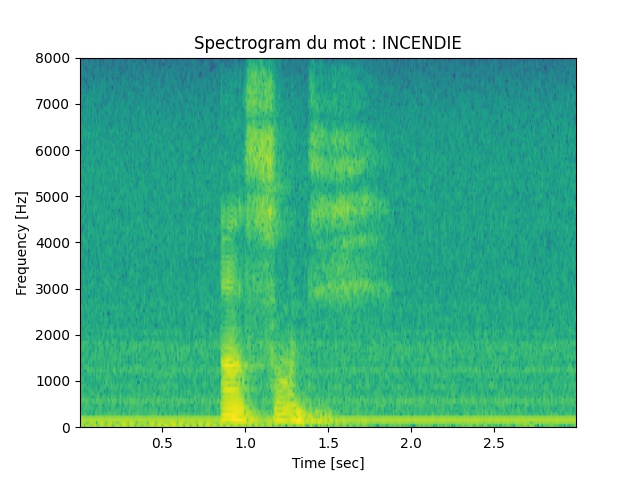
\includegraphics[height=0.20\textheight]{1-Incendie-3.jpg} \\ \hline \\
    2 & L'apprentissage automatique & 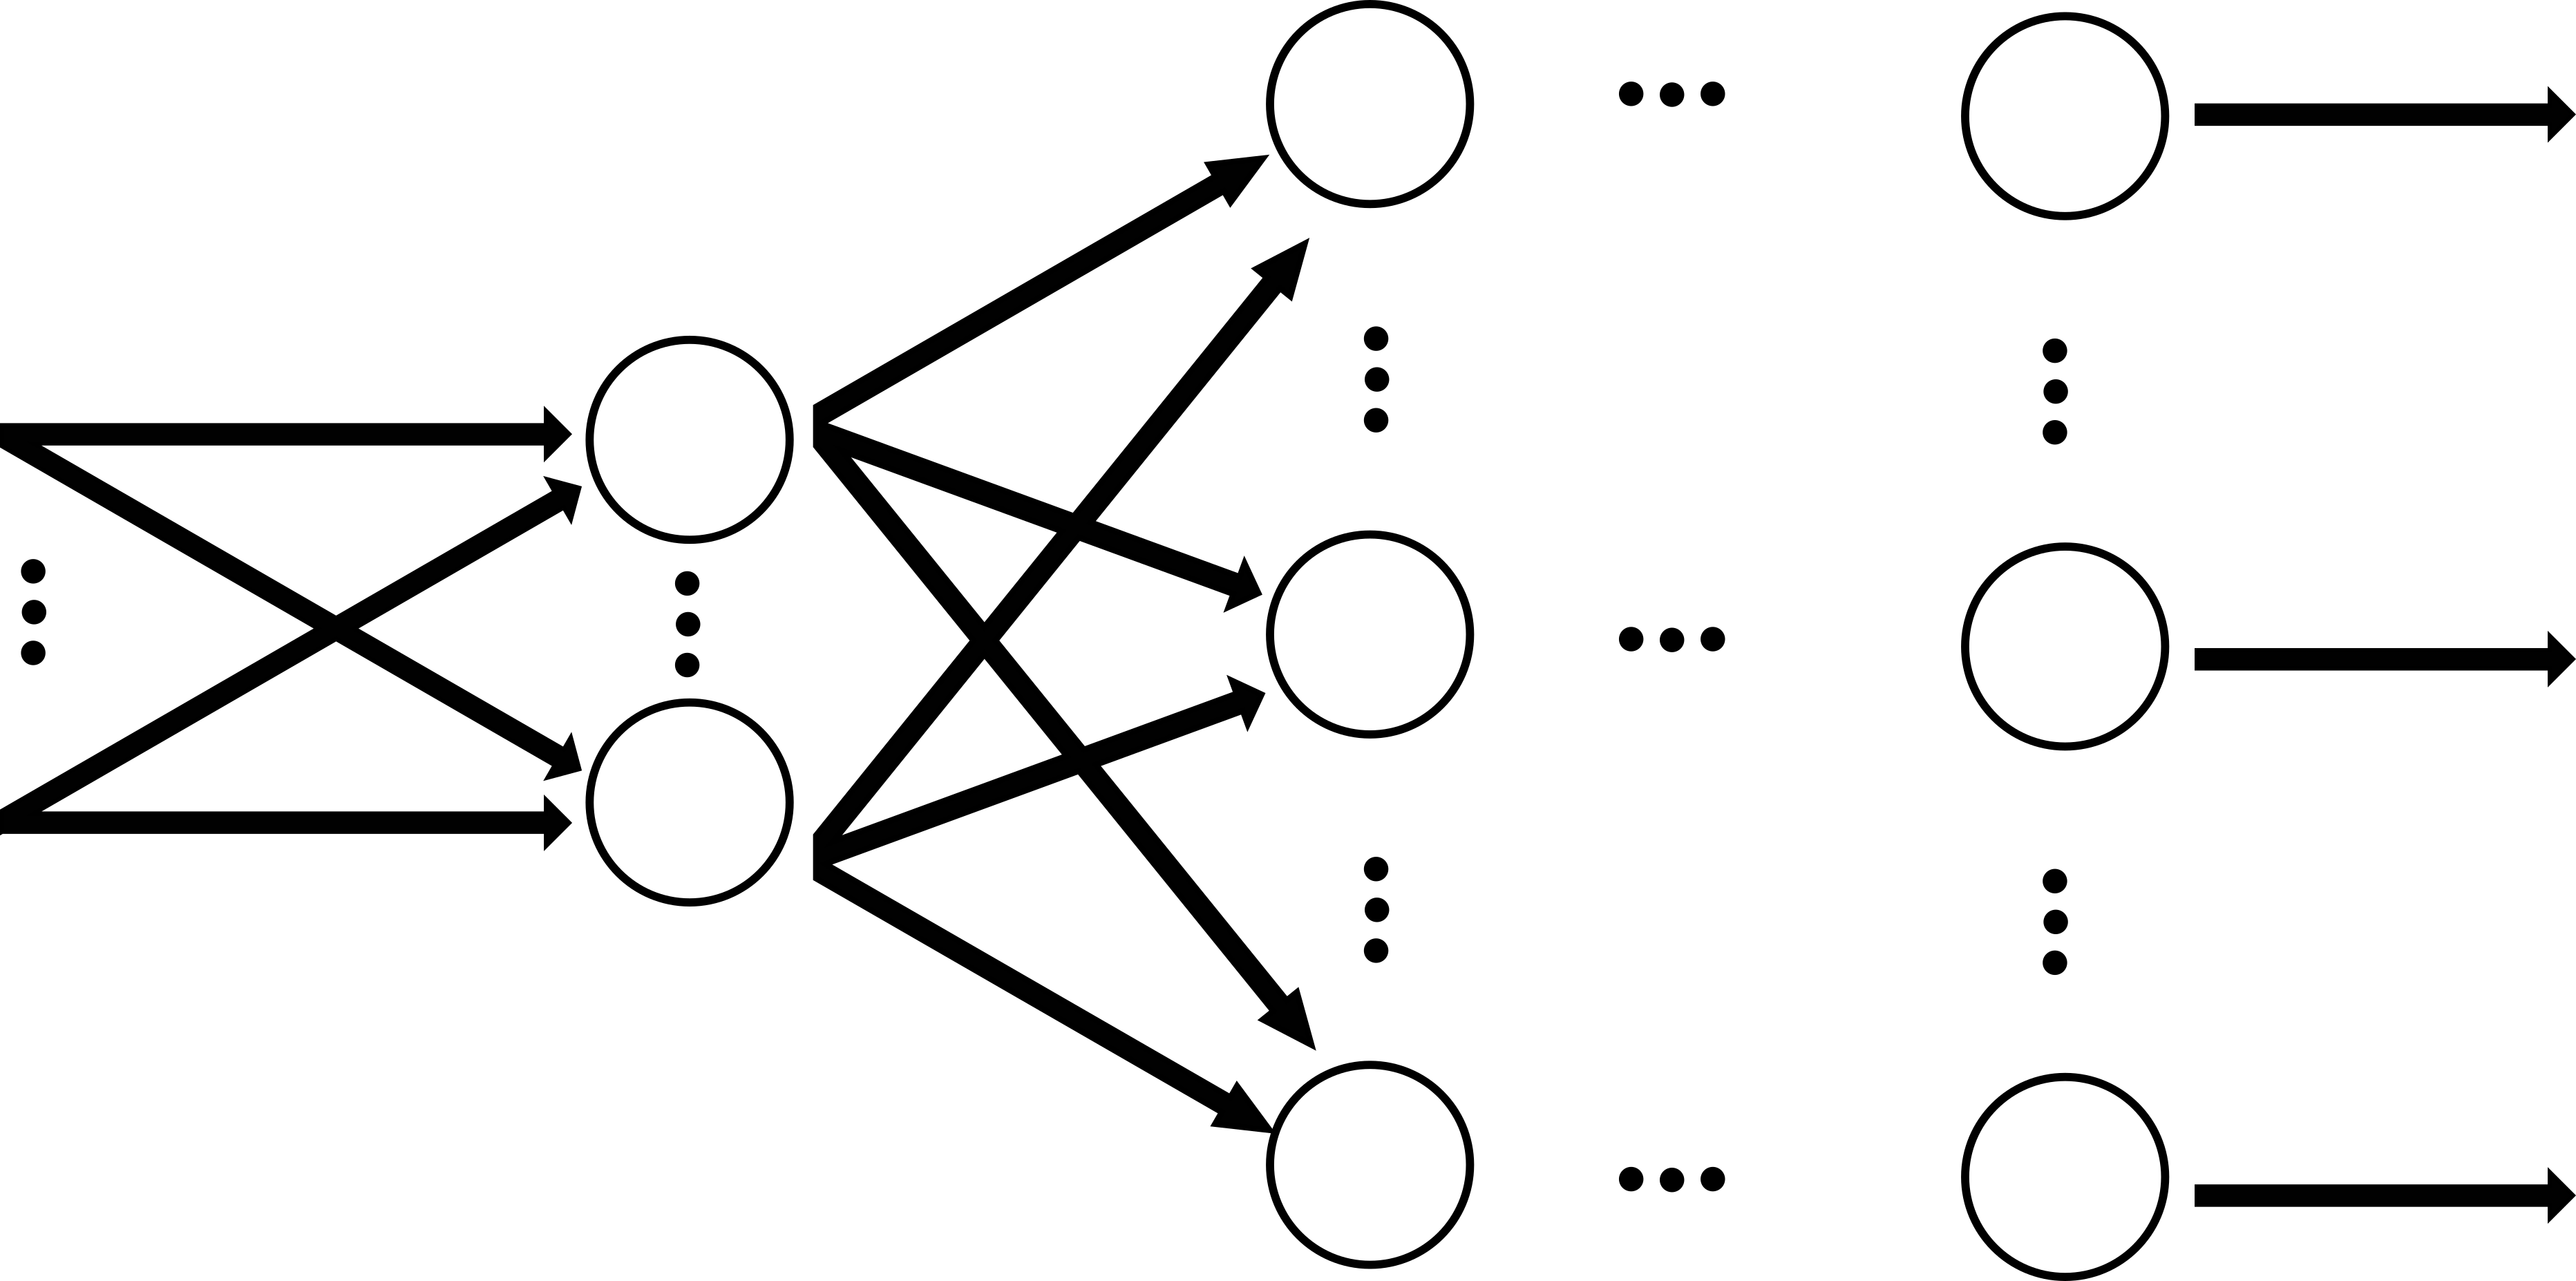
\includegraphics[height=0.20\textheight]{2-Reseau.png} \\ \hline \\
    3 & Le décodage & 
\includegraphics[height=0.20\textheight]{3-Matching.png} \\ \hline
\end{tabular}
\end{frame}



